\documentclass[sigconf,nonacm]{acmart}

\input{includes/preamble_common}
\input{includes/preamble_acm}

\AtBeginDocument{\providecommand\BibTeX{{\sc Bib}\TeX}}

\title[Integración de patrones de diseño]{Integración de patrones de diseño y paradigmas de desarrollo en proyectos de software gestionados con Scrum}

\author{Carlos Francisco Andrade Bermeo}
\affiliation{%
  \institution{Análisis y Desarrollo de Software, SENA}
  \city{}
  \country{Colombia}}
\email{}

\begin{abstract}
El objetivo de este artículo es analizar la integración de patrones de diseño, el modelo-vista-controlador (MVC) y la programación orientada a objetos (POO) en el desarrollo de proyectos de software, destacando su potencial para mejorar la organización y mantenibilidad del sistema. Para alcanzar este propósito, se adoptó un enfoque metodológico aplicado en un proyecto académico, en el cual se implementaron dichas prácticas como base en la construcción del sistema. Aunque no se implementó de manera estricta la metodología Scrum, se incorporaron algunas de sus prácticas, como las reuniones diarias, que permitieron evaluar sus beneficios en la gestión ágil y la comunicación entre los integrantes del equipo. Los resultados obtenidos evidencian que la combinación de MVC y POO facilita la separación de responsabilidades y la reutilización del código, mientras que la integración parcial de Scrum potencia la organización colaborativa. Se concluye que este tipo de integración representa un ejemplo de prácticas modernas en el desarrollo de software, aplicables tanto en contextos académicos como profesionales.

\end{abstract}

\keywords{Patrones de diseño, Programación Orientado a Objetos, Scrum, Modelo Vista Controlador}

\begin{document}
\maketitle

\section{Introducción}
El desarrollo de software contemporáneo enfrenta retos significativos, principalmente derivados de la creciente complejidad, escalabilidad y mantenibilidad de los sistemas. Estos desafíos impactan directamente en la calidad del código y su evolución a lo largo del tiempo. En este sentido, \cite{vera2022arquitectura} afirma que, sin una arquitectura de software adecuada, el desarrollo pierde efectividad, ya que la falta de organización afecta negativamente el ciclo de vida del software.

Para abordar estas problemáticas, la comunidad técnica y académica ha promovido la adopción de paradigmas y estructuras de diseño que fomentan la separación de responsabilidades y la reutilización del código. Según \cite{gavilanez2022analisis}, afirma que el paradigma de la Programación Orientada a Objetos (POO) se apoya en patrones de diseño y arquitecturas específicas como el Modelo-Vista-Controlador (MVC), las cuales buscan imponer modularidad, coherencia y claridad en el desarrollo.

De manera complementaria, los equipos de desarrollo han incorporado metodologías ágiles, destacando especialmente Scrum como marco de gestión de proyectos. Según \cite{marco2022revision} y \cite{merchan2022comparacion}, esta metodología propone ciclos iterativos cortos que favorecen la mejora continua, la entrega constante de valor y una comunicación más eficiente entre los miembros del equipo.

En este contexto, el presente trabajo busca analizar y aplicar estas prácticas tanto a nivel técnico como metodológico, con el objetivo de demostrar que la integración de arquitecturas de software bien estructuradas junto con marcos de trabajo ágiles favorece la creación de sistemas más robustos, mantenibles y alineados con las necesidades del cliente.
\section{Marco teórico y trabajos relacionados}
\subsection{A. Patrón de diseño}
Los patrones de diseño constituyen soluciones ya probadas y estructuradas para problemas recurrentes en el desarrollo de software. Su objetivo principal es evitar la duplicación de código y favorecer su reutilización, aportando al mismo tiempo claridad y modularidad en los sistemas. De acuerdo con \cite{gavilanez2022analisis} afirma que los patrones de diseño permiten mantener una lógica de organización en el código, lo cual facilita la creación de software de calidad, con mayor facilidad de mantenimiento y una mejor comprensión por parte de otros desarrolladores. Además, brindan beneficios como la estandarización de soluciones, la reducción de errores comunes y la optimización de tiempos de desarrollo.

\subsection{B. Metodología}
Una metodología, según \cite{merchan2022comparacion}, puede definirse como el conjunto de procesos, habilidades, procedimientos y documentación de apoyo que guían a los desarrolladores en la implementación de nuevos sistemas de información. Estas metodologías se estructuran en sub-fases que funcionan como una hoja de ruta para la planificación, gestión, control y evaluación de los proyectos. Su propósito es proporcionar un marco de trabajo que oriente la selección de las tecnologías más adecuadas en cada etapa del desarrollo, garantizando así un proceso más organizado, eficiente y alineado con los objetivos del sistema.

\subsection{C. Arquitectura de software}
La arquitectura de software se concibe como la estructura fundamental de un sistema, conformada por sus componentes, las interacciones entre ellos y las propiedades que guían su funcionamiento. Más allá de definir cómo se organiza el código, su importancia radica en que establece un marco de referencia que facilita la escalabilidad, el mantenimiento y la comprensión global del sistema. En este sentido, \cite{vera2022arquitectura} señala que, sin una arquitectura bien definida, el desarrollo pierde efectividad, ya que la falta de organización dificulta la claridad y la evolución del software en el tiempo.

\subsection{D. Programación Orientado a Objetos}
La Programación Orientada a Objetos (POO) constituye un paradigma que busca modelar el mundo real de una manera más cercana a la lógica humana. Según \cite{vera2022arquitectura}, este enfoque introduce principios como el encapsulamiento y la abstracción, los cuales permiten la creación de unidades denominadas clases, favoreciendo la reutilización del código y un mejor entendimiento del mismo. Asimismo, \cite{vera2022arquitectura} sostiene que la POO aporta ventajas significativas al permitir la resolución de problemas a partir de códigos ya funcionales, evitando la duplicidad y promoviendo la eficiencia en el desarrollo de sistemas. Este paradigma involucra la definición de clases, objetos, propiedades y métodos, lo que facilita la implementación y organización de los programas, además de mejorar la mantenibilidad y escalabilidad de los proyectos de software.

\subsection{E. Modelo-Vista-Controlador (MVC)}
El patrón Modelo-Vista-Controlador (MVC) surge con el propósito de reducir el esfuerzo en la programación y estandarizar el diseño de aplicaciones que requieren manejar múltiples vistas sincronizadas con los mismos datos \cite{zambrano_patron}. Esta arquitectura organiza una aplicación en tres componentes principales: el Modelo, encargado de la gestión de datos y la lógica de negocio; la Vista, que define la interfaz de usuario; y el Controlador, que actúa como intermediario entre ambos, gestionando las interacciones y solicitudes del usuario. Esta separación favorece la actualización y el mantenimiento del software de manera más sencilla y en menor tiempo, al permitir trabajar de forma independiente en cada componente \cite{zambrano_patron}. De acuerdo con \cite{gavilanez2022analisis}, entre las principales ventajas del MVC destacan la posibilidad de modificar fácilmente un componente sin afectar los demás, la reutilización del modelo para construir diversas vistas sin necesidad de alterarlo, y la facilidad para implementar pruebas unitarias. En conjunto, estas características hacen del MVC promueve la escalabilidad y la eficiencia en el desarrollo de sistemas de software.

\subsection{F. Scrum}
Scrum es una metodología ágil de gestión de proyectos que busca optimizar los procesos de desarrollo mediante ciclos iterativos e incrementales. Según [2], esta metodología se caracteriza por organizar el trabajo en sprints o iteraciones cortas, en las que se definen objetivos específicos y medibles, lo que permite evaluar avances constantes y realizar ajustes oportunos. Dentro de este marco, los roles como el Scrum Master y el Product Owner son esenciales para garantizar la correcta distribución de tareas, la resolución de problemas y la alineación del equipo hacia los objetivos del proyecto.
\section{Metodología de investigación aplicada}
El presente proyecto se desarrolló bajo un enfoque cualitativo, orientado a la comprensión e interpretación de conceptos relacionados con la Programación Orientada a Objetos (POO), el patrón Modelo-Vista-Controlador (MVC) y la metodología ágil Scrum. Estos enfoques metodológicos y arquitectónicos ya habían sido definidos desde el inicio del proyecto formativo como parte de la estrategia de desarrollo del sistema de gestión de eventos.

Sin embargo, con el fin de sustentar y validar teóricamente estas elecciones, se procedió a la búsqueda, selección y análisis de artículos científicos que aportaran evidencia sobre sus beneficios y buenas prácticas en el ámbito del desarrollo de software.

\subsection{A. Fase 1- Recolección y construcción del thesaurus}
• Se utilizó como base de datos Google Scholar, realizando consultas con palabras clave relacionadas: patrones de diseño, MVC, POO, Scrum, metodologías ágiles.
• Cada artículo relevante fue documentado en un archivo "Thesaurus" con campos estandarizados: término, fecha, fuente, nombre del artículo.
• El propósito de esta fase fue reunir evidencia científica que respalde el uso de las tecnologías y metodologías seleccionadas en el proyecto formativo.

\subsection{B. Fase 2- Análisis cualitativo de la evidencia (síntesis del thesaurus)}
• El objetivo fue transformar la información documental en argumentos sólidos que justificaran el uso de MVC, POO y Scrum en el desarrollo del sistema, para ello se realizaron lecturas críticas, resúmenes y reflexiones de los artículos, identificando ahí mismo la separación de responsabilidades, mantenibilidad y el trabajo colaborativo en equipos ágiles.
• La evidencia encontrada reforzó la pertinencia de las decisiones iniciales del proyecto y aportó lineamientos prácticos para guiar el diseño e implementación del sistema.
\input{sections/04_implementacion}
\section{Evaluación y resultados}
Una vez finalizada la fase de análisis cualitativo, se concluyó que el desarrollo de un sistema requiere de una arquitectura sólida sustentada en un paradigma adecuado, lo que garantiza organización del software. Asimismo, en el ámbito del agilismo, se evidenció la importancia de emplear una metodología debidamente estructurada, como Scrum, que permita adaptarse a los cambios, mejorar la comunicación entre los participantes del proyecto y facilitar la entrega incremental de funcionalidades. Estos hallazgos no solo orientaron las decisiones técnicas adoptadas en el proyecto formativo, sino que también aportaron criterios prácticos para optimizar la colaboración del equipo y la calidad del producto desarrollado. A partir de esto se obtuvieron resultados relevantes en tres planos:

\subsection{1. Resultados en la arquitectura y el desarrollo del sistema}
Se obtuvo un software basado en la arquitectura Modelo-Vista-Controlador (MVC), la cual permitió separar las responsabilidades en capas (modelo, vista y controlador), favoreciendo la organización del código. De manera complementaria, la adopción de la Programación Orientada a Objetos (POO) aportó principios como la reutilización, el encapsulamiento y la escalabilidad, lo que garantizó un desarrollo más estructurado y con mayor facilidad para la mantenibilidad y evolución futura del sistema.

\begin{figure}[htbp]
    \centering
    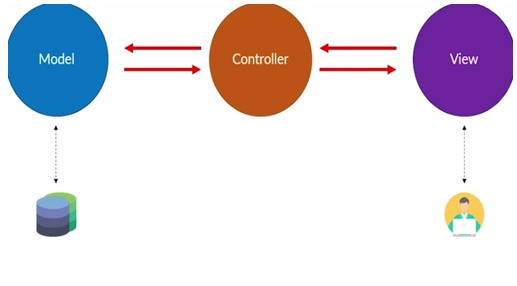
\includegraphics[width=0.8\textwidth]{graphics/mvc.jpeg}
    \caption{Modelo vista controlador}
    \label{fig:mvc}
\end{figure}

En la Figura \ref{fig:mvc} se ilustra la estructura de la arquitectura Modelo–Vista–Controlador (MVC) adoptada en el desarrollo del sistema de gestión de eventos. El uso de MVC permitió que cada componente pudiera desarrollarse y mantenerse de forma independiente, garantizando un código más organizado y facilitando la incorporación de nuevas funcionalidades sin afectar el resto del sistema.

\subsection{2. Resultados en la aplicación de la metodología ágil (Scrum)}
La implementación de la metodología ágil Scrum en el desarrollo del sistema generó beneficios tanto en el ámbito técnico como en el fortalecimiento de las habilidades blandas del equipo. En el plano técnico, permitió una adecuada planificación, control y seguimiento de los avances mediante la organización en sprints, lo que facilitó la adaptación a cambios y la entrega incremental de funcionalidades. En el plano humano, fomentó la comunicación constante, la colaboración y la responsabilidad compartida, promoviendo un ambiente de trabajo más dinámico y orientado a la resolución conjunta de problemas.

\begin{figure}[htbp]
    \centering
    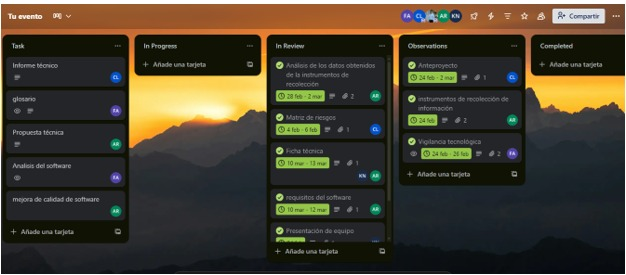
\includegraphics[width=0.8\textwidth]{graphics/trello.jpeg}
    \caption{Tablero trello}
    \label{fig:trello}
\end{figure}

En la Figura \ref{fig:trello} se observa el tablero de Trello empleado para la planificación y seguimiento de los sprints. Este recurso permitió visualizar las tareas pendientes, en progreso y completadas, facilitando la comunicación del equipo y el control de avances bajo la metodología ágil Scrum.
\input{sections/06_discusion}
\section{Conclusiones y trabajo futuro}
A partir de la metodología cualitativa implementada en este proyecto, se evidenció que la combinación de una arquitectura sólida y una metodología ágil resulta fundamental para el éxito en el desarrollo de sistemas. La revisión documental mediante el thesaurus permitió identificar conceptos clave como la Programación Orientada a Objetos (POO), el patrón Modelo–Vista–Controlador (MVC) y la metodología Scrum, los cuales aportaron lineamientos claros y prácticos para la construcción del sistema de gestión de eventos.

Los resultados obtenidos demuestran que la aplicación de MVC y POO facilita la organización, escalabilidad y mantenibilidad del software, mientras que el uso de Scrum fortaleció la comunicación del equipo, la planificación de tareas y la entrega incremental de funcionalidades. En conjunto, estos hallazgos confirmaron que la investigación documental y la práctica de desarrollo estuvieron alineadas, logrando así un proyecto formativo con bases teóricas sólidas y un producto funcional que responde a las necesidades planteadas.
\input{sections/A1_apendices}

\bibliographystyle{ACM-Reference-Format}
\bibliography{bibliography/references}

\end{document}